\documentclass[12pt,a4paper]{article}

%\pdfoutput=1

\usepackage[utf8]{inputenc}
\usepackage[T1]{fontenc}
\usepackage[english]{babel}
\usepackage{amsmath}
\usepackage{mathabx}
\usepackage{lmodern}
\usepackage{units}
\usepackage{siunitx}
\usepackage{icomma}
\usepackage{graphicx}
\usepackage{caption}
\usepackage{subcaption}
\usepackage{color}
\usepackage{pgf}
\DeclareMathOperator{\acosh}{arccosh}
\newcommand{\N}{\ensuremath{\mathbbm{N}}}
\newcommand{\Z}{\ensuremath{\mathbbm{Z}}}
\newcommand{\Q}{\ensuremath{\mathbbm{Q}}}
\newcommand{\R}{\ensuremath{\mathbbm{R}}}
\newcommand{\C}{\ensuremath{\mathbbm{C}}}
\newcommand{\rd}{\ensuremath{\mathrm{d}}}
\newcommand{\id}{\ensuremath{\,\rd}}
\usepackage{hyperref}
%\usepackage{a4wide} % puts the page numbering further down the page.
\usepackage{pdfpages}
\usepackage{epstopdf}
\DeclareGraphicsExtensions{.eps}

\title{Handin 1: Extraction of extrinsic parameters.}
\author{Marcus Malmquist, marmalm, 941022}
\date{\today}

\begin{document}
\maketitle

\section{Task 1}\label{sec:1}
In this section I describe the method I used to extract the values of the extrinsic components. This method was proposed by Dambrine and Gao.

\subsection{Extrinsic resistances and inductances}\label{sec:1a}
The equations (proposed by Dambrine) used to extract the parasitic resistances and inductances at the gate, drain and source can be seen in (\ref{eq:rl_eqs}). Some necessary values can be seen in Figure~\ref{fig:rl_fig}.
\begin{equation}
  \label{eq:rl_eqs}
  \mathbf{Z}=
  \begin{bmatrix}
    R_s+R_g+\frac{R_c}{3}+\frac{nkT}{qI_g}+j\omega(L_s+L_g) & R_s+\frac{R_c}{2}+j\omega L_s \\
    R_s+\frac{R_c}{2}+j\omega L_s & R_s+R_d+j\omega(L_s+L_d)
  \end{bmatrix}
\end{equation}
The matrix $\mathbf{Z}$ can be found by conversion from the scattering matrix $\mathbf{S}$. The values of $R_g$, $R_d$, $R_s$, $L_g$, $L_d$ and $L_s$ can be seen inductances Figure~\ref{fig:rl_fig}.
\begin{figure}
  \centering
  \noindent\makebox[\textwidth]{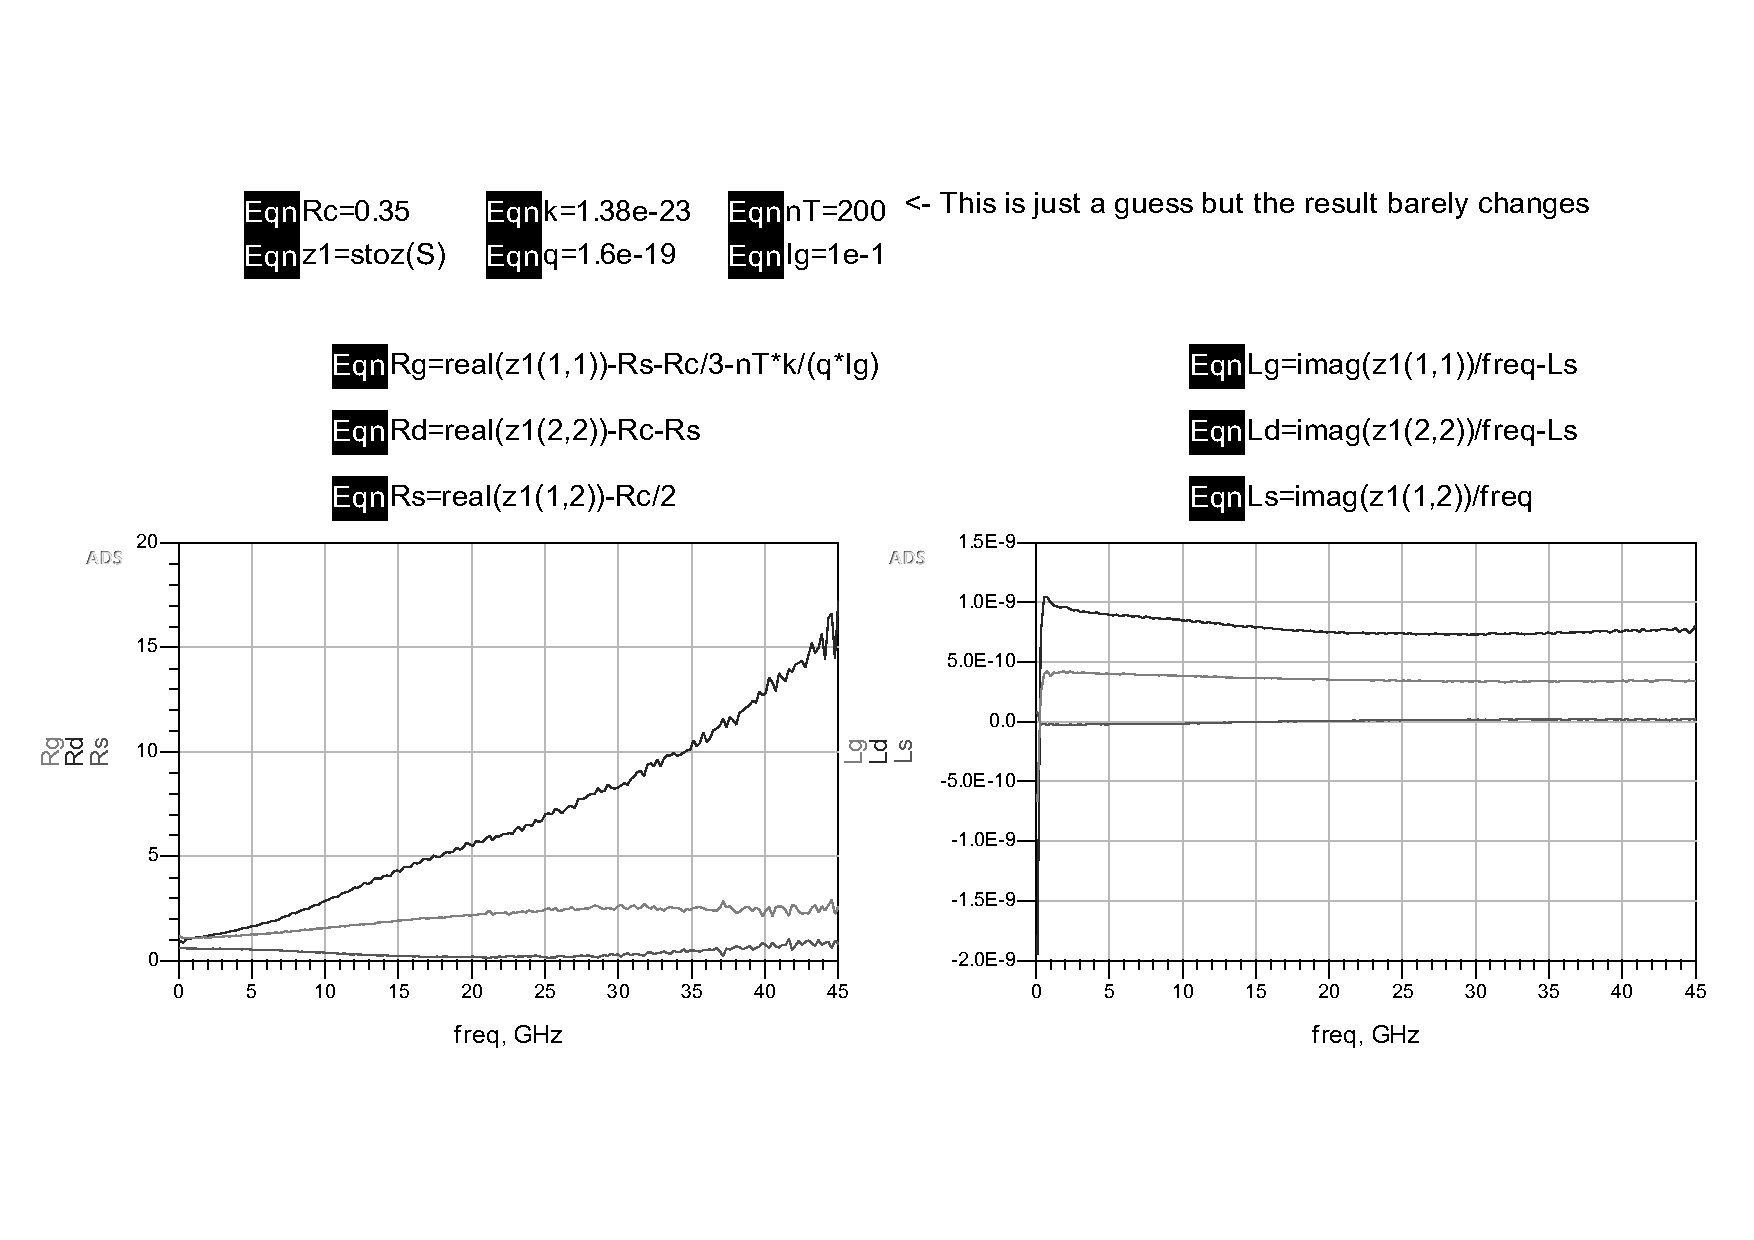
\includegraphics[width=\textwidth]{cold_fet_forward_bias.pdf}}
  \caption{The extrinsic resistances and inductances plotted versus the frequency.}
  \label{fig:rl_fig}
\end{figure}

\subsection{Extrinsic capacitances}\label{sec:1b}
The equations (proposed by Gao) used to extract the parasitic capacitances between gate and source, drain and source as well as gate and drain can be seen in (\ref{eq:c_eqs}). Some necessary values can be seen in Figure~\ref{fig:c_fig}.
\begin{equation}
  \label{eq:c_eqs}
  \mathbf{Y}=
  \begin{bmatrix}
    \omega(C_{\text{pg}}+C_{\text{pgd}}+W(C_{\text{gspo}}+C_{\text{gdpo}})) & -\omega(C_{\text{pgd}}+WC_{\text{gdpo}}) \\
    -\omega(C_{\text{pgd}}+WC_{\text{gdpo}}) & \omega(C_{\text{pd}}+C_{\text{pgd}}+W(C_{\text{dspo}}+C_{\text{gdpo}}))
  \end{bmatrix}
\end{equation}
The matrix $\mathbf{Y}$ can be found by conversion from the scattering matrix $\mathbf{S}$. The values of $C_{\text{pg}}$, $C_{\text{pgd}}$ and $C_{\text{pgd}}$ can be seen in Figure~\ref{fig:c_fig}.
\begin{figure}
  \centering
  \noindent\makebox[\textwidth]{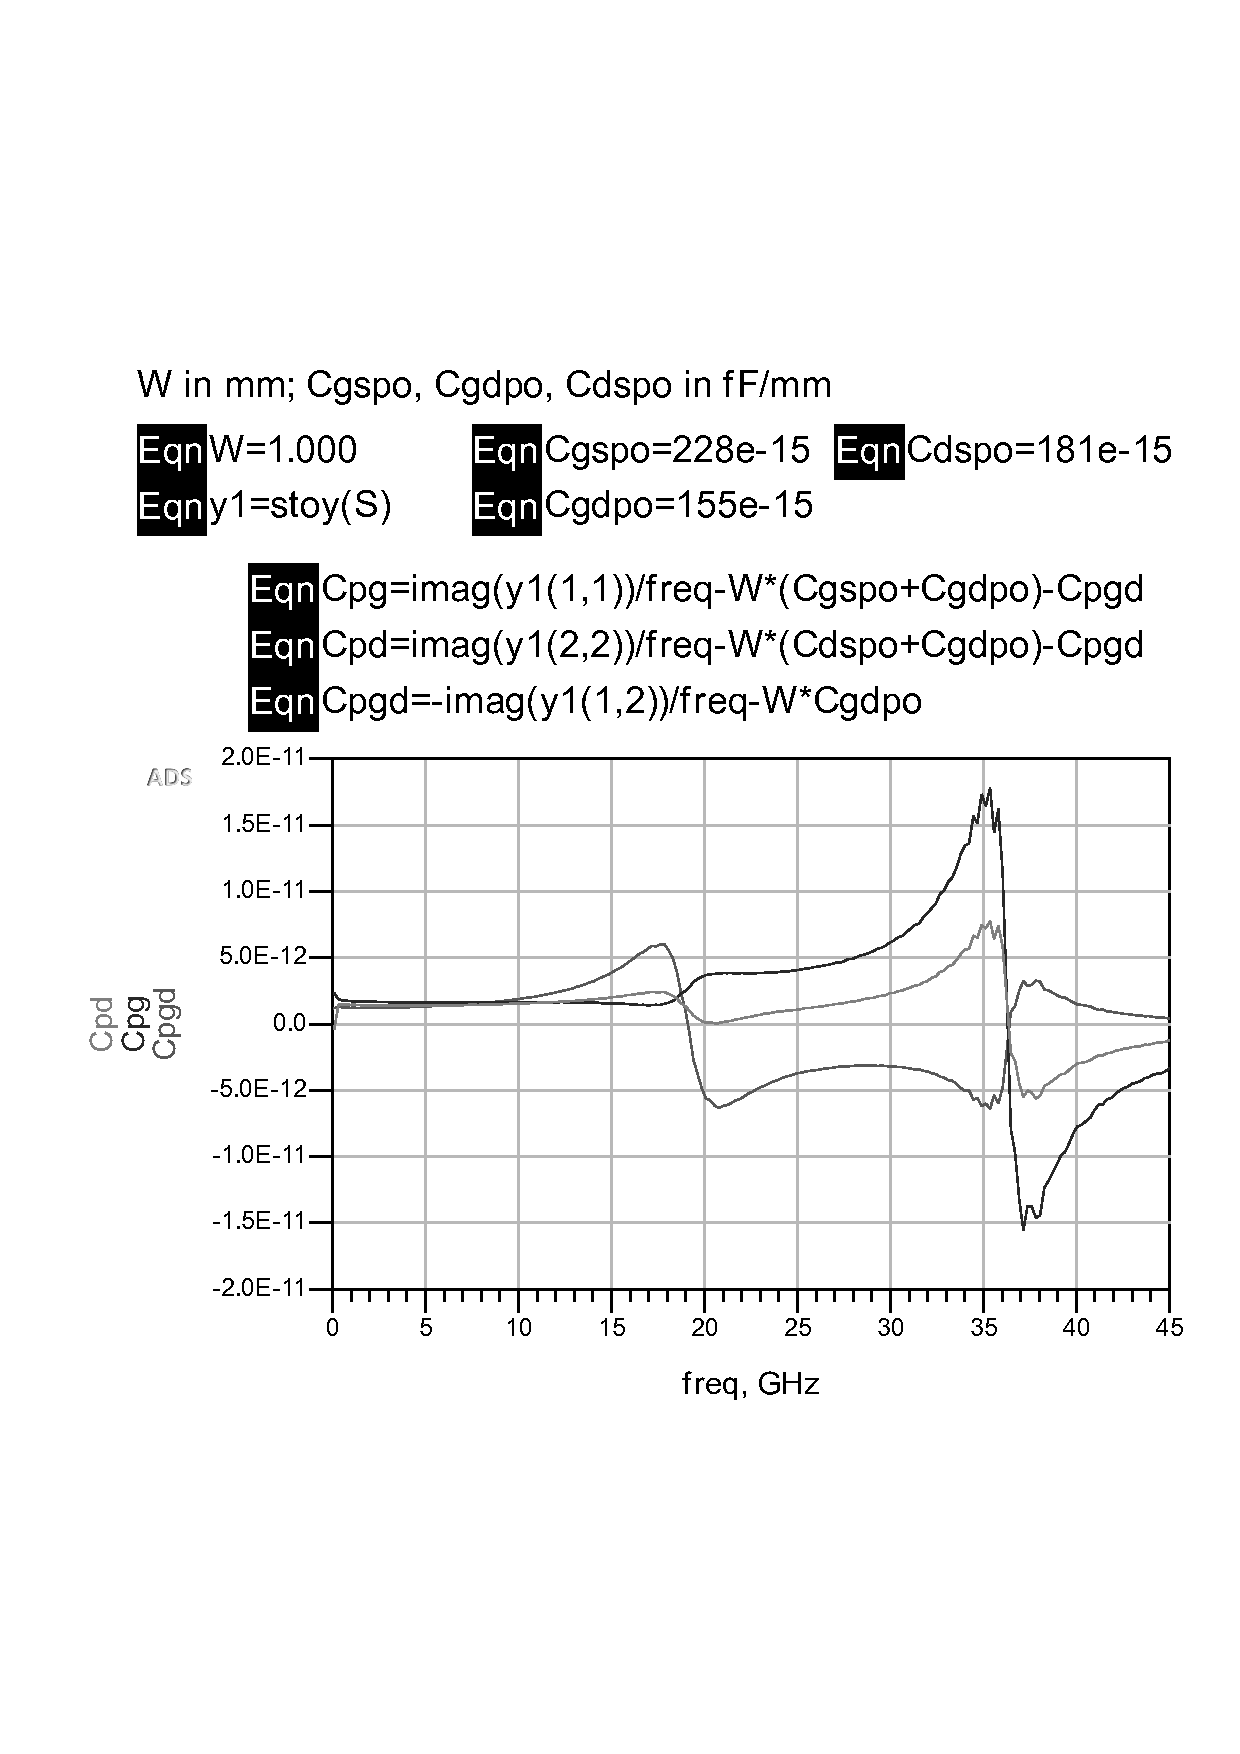
\includegraphics[width=\textwidth]{cold_fet_pinchoff_bias.pdf}}
  \caption{The extrinsic resistances and inductances plotted versus the frequency.}
  \label{fig:c_fig}
\end{figure}
\end{document}